\chapter{Estado de la Cuestión}
\label{cap:estadoDeLaCuestion}
En este capítulo se hará una investigación sobre las técnicas, herramientas y formas de crear inteligencias artificiales para enemigos.
Para ello vamos a comenzar haciendo un recorrido por todo lo relacionado con la inteligencia artificial en general y cómo se usa esta en videojuegos 2D de plataformas, ya sea para crear un NPC, un enemigo o para optimizar alguna función más a bajo nivel del juego.
Se mencionarán además herramientas para conseguir los fines descritos anteriormente y se hablará de algunos motores de videojuegos que han inspirado en cierta manera algunos aspectos de nuetras herramienta. \\
\section{Introducción a la Inteligencia Artificial}

La Inteligencia Artificial (IA) es la capacidad que tiene un sistema o software de realizar tareas diferentes entre sí de manera autónoma aplicando reglas, algoritmos o patrones de aprendizaje automático, simulando así comportamientos propios de la inteligencia humana.
El potencial de la IA hoy día y por lo que está generando tanto furor es su capacidad de autonomía, ya que no solo sigue reglas, si no que tiene la capacidad de tomar decisiones\\
En el ámbito de los videojuegos, la IA se ha hecho paso a base de demostrar su gran capacidad de adaptación a contextos diversos como la adaptación del Alien en \textit{Alien Isolation}\footnote{\url{https://www.gamedeveloper.com/design/the-perfect-organism-the-ai-of-alien-isolation}} , la manera en la que puede generar contenido procedural para juegos roguelike como \textit{Hades}\footnote{\url{https://hades.fandom.com/es/wiki/Hades_(juego)}} o ,por último, entrenar una IA para que se acerque lo máximo posible al comportamiento de un humano como en la serie \textit{Forza Motosport}\footnote{\url{https://forza.fandom.com/wiki/Forza_Wiki}}, usando redes neuronales.\\
\section{Tecnicas}

Es muy importante a la hora de escoger una técnica para modelar la IA de una entidad el saber ciertos factores para tomar la decisión correcta, como por ejemplo la complejidad esperada del comportamiento, la escalabilidad y flexibilidad de la técnica, si queremos invertir mucho tiempo en implementar estas técnicas o queremos algo rápido de hacer y funcional, los recursos que consumen... \\

A continuación, se presentarán una serie de técnicas que se usan en los videojuegos para crear IAs.
\subsection{Maquinas de estado finitas}
Las máquinas de estado finitas, en inglés finite state machine, con siglas FSM, son un modelo matemático que representan un número finito de estados y una serie de transiciones entre ellos. \\

Una FSM se representa como un grafo, siendo este una representación abstracta de un conjunto de objetos, eventos, acciones o propiedades conectados entre sí, siendo estos elementos nodos (estados) que realizan acciones y comprueban la posibilidad de que haya que cambiar de nodo. 

En el ámbito de los videojuegos, las FSM son el conjunto de estados que puede tomar una entidad y la forma de llegar a estos, teniendo en cuenta que solo puede haber un estado activo en cualquier instante. \\

El primer videojuego documentado que utilizó FSM para implementar la lógica de juego fue \textit{Spacewar!(1961)}\footnote{\url{https://www.ijarsct.co.in/Paper2062.pdf}} desarrollado en el MIT por Steve Russell. Este videojuego implementaba una lógica basada en estados para manejar el comportamiento de las naves, la detección de colisiones y la física del juego. Aunque no usaba una implementación formal de máquinas de estado, sí modelaba cambios entre estados bien definidos, como el movimiento de las naves o la activación de los disparos. \\ 

\textit{Pac-Man}\footnote{\url{https://pacman.fandom.com/es/wiki/Pac-Man_Wiki:Portada}} es un videojuego en el que el jugador controla un personaje amarillo en forma de círculo con una boca que se abre y cierra constantemente y fue lanzado en 1980 por la compañía japonesa Namco (actual Bandai Namco). El objetivo de este videojuego es el de recorrer un laberinto e ir comiendo todos los puntos mientras evitamos cuatro fantasmas hasta que comemos una píldora de poder que nos hace invulnerable y nos da la capacidad de comer a los fantasmas. Estos huirán tras comernos la píldora.\\\\
La complejidad en la IA de Pac-Man es asombrosa ya que se le quiso dar profundidad al juego haciendo que cada fantasma tuviera una personalidad diferente. Para ello se implementó una máquina de estado por fantasma haciendo que la forma en la que estos interactúan con el entorno sea ligeramente diferente.
A continuación se enumerarán los fantasmas y sus formas de comportarse.
\begin{itemize}
	 \item Blinky: es el fantasma rojo y su papel es el de cazador, siendo su personalidad la más agresiva, hecho que se refleja en que es el único fantasma que comienza fuera de la casa de los fantasmas y que tras salir empieza a perseguir al jugador incansáblemente. Tiene otra característica propia, a medida que el jugador va comiendo bolitas, comienza a aumentar su velocidad.
	 \item Pinky: como su nombre indica es el fantasma de color rosa. En japonés se llama \textit Machibuse, el que tiende emboscadas. Pinky es el interceptor del juego por lo que va a tratar de cortar el camino del jugador. Es un fantasma relativamente rápido, por lo que calculará constantemente hacia donde se dirige el jugador para usar su velocidad para adelantarse y cortar el paso.
	 \item Inky: el fantasma azul es el más impredecible de todos, ya que su función es la de adoptar temporalmente la personalidad de sus otros tres compañeros.
	 \item Clyde: el fantasma naranja y el más tranquilo de todos. Suele ser el último en salir de la casa de los fantasmas y no intentará atrapar al jugador a no ser que este esté muy cerca de él. El resto del tiempo deambula por el mapa e intenta evitar al jugador.
\end{itemize}
Para ilustrar el funcionamiento del juego se usará la Figura \ref{fig:Comportamiento jugador Pac-Man} que representa una posible FSM para el jugador, lo que haría que las decisiones tomadas fueran lo más eficientes posibles en el momento.\\

\begin{figure}[h]
	\centering
	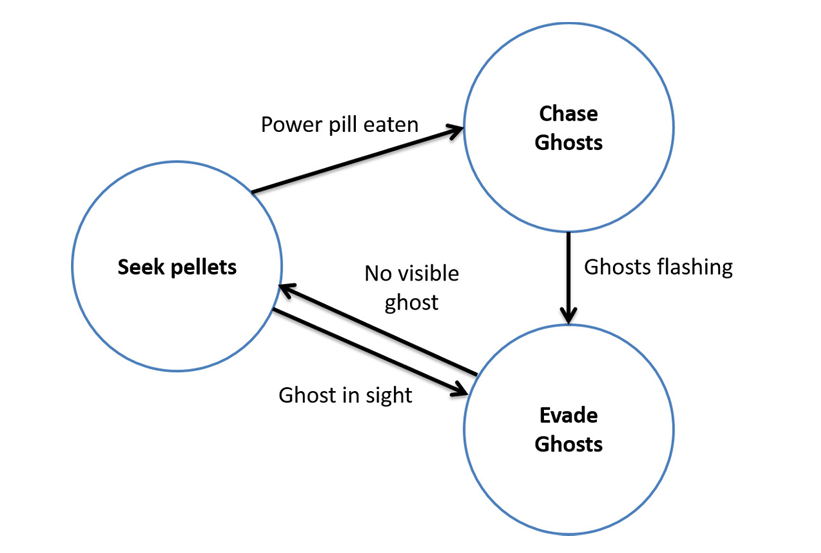
\includegraphics[width = 0.7\textwidth]{Imagenes/FMS_MsPac-man.png}
	\caption{Comportamiento jugador Pac-Man, extraído del libro de Yannakakis y Togelius (2018)}
	\label{fig:Comportamiento jugador Pac-Man}
\end{figure}

Un punto en contra de las FSMs es que son muy inflexibles y estáticas, de manera que las posibilidades de escalado de la lógica son limitadas. También son algo predecibles una vez el jugador ha estudiado los estados y transiciones de una entidad, este punto negativo puede paliarse implementado probabilidades o reglas que no estén tan claras a la hora de hacer las transiciones.

\subsection{Árboles de comportamiento}

Un árbol de comportamiento o Behavior Tree (BT) es un sistema similar a las FSMs ya que contamos con nodos y transiciones y solo uno de esos nodos, que ahora pasan a ser comportamientos en lugar de estados, puede estar activo al mismo tiempo. \\
En esencia, es un árbol de nodos que se organizan jerárquicamente y que atienden a unas normas que controlana el flujo de cambios de nodo. \\

La principal ventaja respecto a las FSMs es su modularidad, la capacidad que tiene un sistema de dividir la lógica del comportamiento en piezas independientes y reutilizables, pudiendo agrupar estas piezas en grupos que a su vez funcionan como una pieza. \\
Su facilidad para ser diseñados y testeados han hecho que los árboles de comportamiento se conviertan en una opción real para modelar IA en la industria del videojuego, con juegos como \textit{Bioshock (2K Games, 2007)}\footnote{\url{https://es.wikipedia.org/wiki/BioShock}} y \textit{Halo 2 (Microsoft Game Studios, 2004)}\footnote{\url{ https://www.gamedeveloper.com/programming/gdc-2005-proceeding-handling-complexity-in-the-i-halo-2-i-ai}} como referencias en el uso de BTs.\\

Un ejemplo no tan conocido de uso de BTs en la industria del videojuego es \textit{Spore (2008, Maxis)}. Spore es un videojuego en el que el jugador va a comenzar creando una célula y va encarnarla durante todo el proceso de su evolución hasta que esta se convierta en un ser mucho más complejo llegando incluso a construir una civilización muy avanzada. La inteligencia artificial de las entidades que nos rodean en este videojuego están fundamentadas en BTs.\\

La gran diferencia de como usa BTs Spore a los juegos anteriormente mencionados es que Spore separa el concepto de \textit{decider} de \textit{behavior}. Los BTs de Halo 2 están compuestos por \textit{behaviors} ya sean estos comportamientos grupales, en los que se elige entre varias opciones, o individuales, que ejecutan acciones específicas, e impulsos que son los saltos que se dan entre comportamientos y que se toman dependiendo de una prioridad, que a futuro resulta en problemas de escalabilidad. Para solucionar este problema, en Maxis deciden unificar el concepto de impulso y comportamientos grupales bajo el nombre de \textit{deciders}, dejando completamente separado el concepto de \textit{behavior} y permitiendo que estos puedan ser reutilizados en múltiples lugares del árbol, asegurando la escalabilidad.\\

La Figura \ref{fig:BT Spore} es un ejemplo de un BT sacado de las documentación\footnote{ \url{https://chrishecker.com/My_Liner_Notes_for_Spore/Spore_Behavior_Tree_Docs}} que hay publicada del juego.
Un punto importante a tener en cuenta es que si un nodo tiene más de un hijo, estos se comprueban si son o no elegidos en un orden determinado hasta que un de los \textit{deciders} acepte la petición del padre o ninguno acepte y se vuelva al nodo actual volviendo a repetir el proceso.\\

\begin{figure}[h]
	\centering
	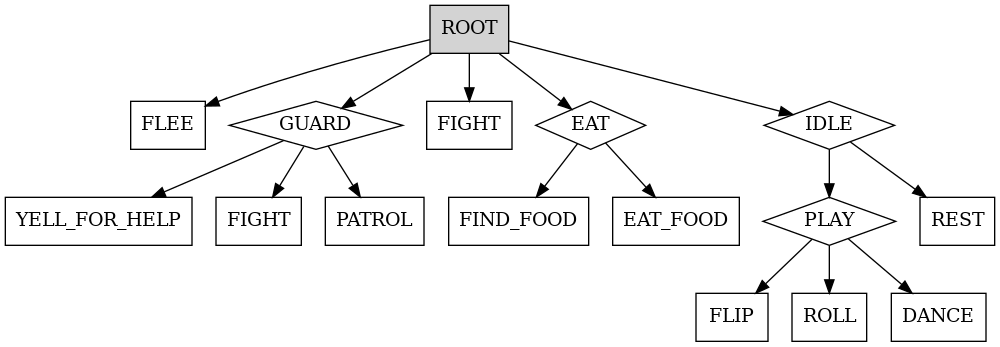
\includegraphics[width = 0.7\textwidth]{Imagenes/BT_Spoore.png}
	\caption{Ejemplo BT, Documentación Spore}
	\label{fig:BT Spore}
\end{figure}
\subsection{Goal-Oriented Action Planning}

GOAP es un sistema basado en planificación de acciones. En lugar de definir comportamientos fijos como hemos visto anteriormente, la entidad analiza la situación y construye un plan óptimo para alcanzar el objetivo designado.
Esta técnica fue desarrollado en el \textit{MIT} por \textit{Jeff Orkin} a principio de siglo. 

La entidad pasa a ser un agente autónomo que tiene la capacidad de planificar de manera dinámica una secuencia de acciones para satisfacer una meta. Para llegar a esa meta se tendrán en cuenta el contexto del agente, por lo que dependiendo de este se podrá llegar a la meta de varias maneras, aunque la utilizada sea la mejor valorada, de esta manera reducimos lo repetitivo que pueda llegar a ser lidiar con un tipo de agente, ya que siendo el enemigo, por ejemplo, el mismo este abordará al jugador de manera distinta dependiendo de la situación que se de.

El enfoque de GOAP es muy parecido a una FSM, pero en GOAP las acciones y metas no van de la mano, si no que se separan para abrir la posibilidad de tener un proceso de planificación dinámico y adaptativo.
La escalabildad  que ofrece GOAP es mayor que todas las técnicas vistas anteriormente.

El considerado primer videojuego que usa GOAP es \textit{F.E.A.R, Monolith Productions}\footnote{\url{https://www.gdcvault.com/play/1013282/Three-States-and-a-Plan}}. El propio Jeff Orkin explica que en el videojuego se quería llegar a una complejidad en la IA a la que las FSMs no podían llegar, por lo que optaron por no excluirlas pero solo tener tres estados y usar un algoritmo A* para planear las acciones a realizar. Un ejemplo es que si el jugador cierra una puerta mientras persigue un enemigo, el enemigo puede dinámicamente volver a rehacer su plan y decidir si buscar un hueco para disparar, por ejemplo una ventana, o buscar una entrada alternativa. Esta libertad en las acciones de los agentes liberan a los desarrolladores para que estos puedan enfocarse en el manejo de grupos, como fuego de supresión, cobertura y búsqueda del jugador.

\citet{GOAP_Jeff_Orkin} nos ofrece otro ejemplo ilustrativo de lo que es GOAP. El videojuego al que se refiere es \textit{NOLF 2}\footnote{\url{https://nolf.fandom.com/wiki/No_One_Lives_Forever_2:_A_Spy_in_H.A.R.M.\%27s_Way}}, siendo este considerado el primer videojuego que usa un sistema parecido a GOAP, los agentes estaban dirigidos por metas aunque no podían planificar sus acciones.
A continuación vamos a definir una serie de términos clave para definir el comportamiento de GOAP.
\begin{itemize}
	 \item Objetivos: lo que la entidad quiera lograr. Un agente puede querer cumplir más de un objetivo. En el videojuego \textit{NOLF 2} los personajes tenían típicamente alrededor de 25 objetivos, aunque en cada instante solo un objetivo esté activo y este determine las acciones del agente. Un objetivo sabe como calcular su relevancia actual y sabe cuando ha sido alcanzado.\\
Aunque conceptualmente son similares, hay una diferencia clave entre los objetivos en \textit{NOLF 2} y GOAP y es que en el primero cada objetivo tiene un plan predefinido con pasos fijos y ramas condicionales establecidas de antemano y en GOAP los objetivos solo definen las condiciones que deben cumplirse para darse por terminado, los pasos para alcanzarlos se generan dinámicamente en tiempo real.

	 \item Plan: forma de denominar una secuencia de acciones. Un plan válido es aquel que lleva a un personaje desde un estado inicial hasta un estado que cumple con el objetivo. El plan se ejecuta hasta que se complete, se invalide u otro objetivo se vuelva más importante lo que obligará a que se cree formule un nuevo plan.
Hay que tener en cuenta que GOAP necesita el funcionamiento de las FSMs y las simplifica enormemente, teniendo esto en cuenta, un plan es también una secuencia de acciones donde cada acción representa una transición entre dos estados.

	 \item Acción: una acción es un paso único y atómico dentro de un plan que hace que un personaje haga algo. Algunas acciones posibles en \textit{NOLF 2} es \textit{Go To Point}, \textit{Draw Weapon}...
La duración de una acción puede variar, por ejemplo la acción \textit{Reload Weapon} terminará cuando la acción acabe, mientras que la acción \textit{Attack} puede continuar indefinidamente hasta que el objetivo muera.\\
Cada acción determina cuándo puede ejecutarse y qué impacto tendrá en el mundo del juego, es decir una acción conoce sus \textit{precondiciones} y sus \textit{efectos}.
	
	\item Mundo: estado actual del contexto de la entidad.
 	
	\item Planificador: encuentra la secuencia óptima de acciones para lograr el objetivo partiendo del estado actual del agente. Si tiene éxito devolverá un plan que el personaje seguirá para guiar su comportamiento.\\
Para ilustrar el funcionamiento del planificador usaremos la Figura \ref{fig:GOAP_Planificador}.
Los rectángulos representan el estado inicial y el estado objetivo, los círculos representan las acciones disponibles.
En este caso, el objetivo es matar a un enemigo, por lo que el estado final es aquel en el que el enemigo está muerto, en otras palabras, el planificador tiene que encontrar una secuencia de acciones que tome el mundo desde un estado en el que el enemigo está vivo hasta otro en el que este está muerto.\\
Este proceso se aborda como un \textit{pathfinding}. El planificador tiene que encontrar un plan válido y no siempre este es el esperado por el usuario. Para ello debemos darle ciertos requisitos al algoritmo de \textit{pathfinding}, por ejemplo, encontrar la secuencia de acciones más baratas que nos lleven al objetivo.


	
	
\end{itemize}
\comp{https://github.com/crashkonijn/GOAP herramienta que podriamos analizar}\\ 
\section{Análisis herramientas}

Tras abordar algunas técnicas usadas para crear IAs, se ha visto que en algunas ocasiones la complejidad de crear esas IAs no es del todo trivial. Por ello, surge la necesidad de crear herramientas que ayudasen a los desarrolladores a crear IAs de todo tipo. Teniendo en cuenta que la creación de IAs debe estar al alcance de personas con nulo conocimiento de programación, estas herramientas deben implementar una interfaz gráfica para que el funcionamiento de la IA sea más visual.
A continuación, se han seleccionado algunas herramientas como ejemplo.\\

\subsection{Behavior Bricks}

\textit{Behavior Bricks}\footnote{\url{https://bb.padaonegames.com/doku.php}} es una herramienta disponible para el motor de videojuegos \textit{Unity} centrada en cubrir todas las necesidades de implementación de comportamientos para juegos. Con \textit{Behavior Bricks} el usuario es capaz de modelar de manera visual tanto FSMs como BTs.\\
\begin{figure}[h]
	\centering
	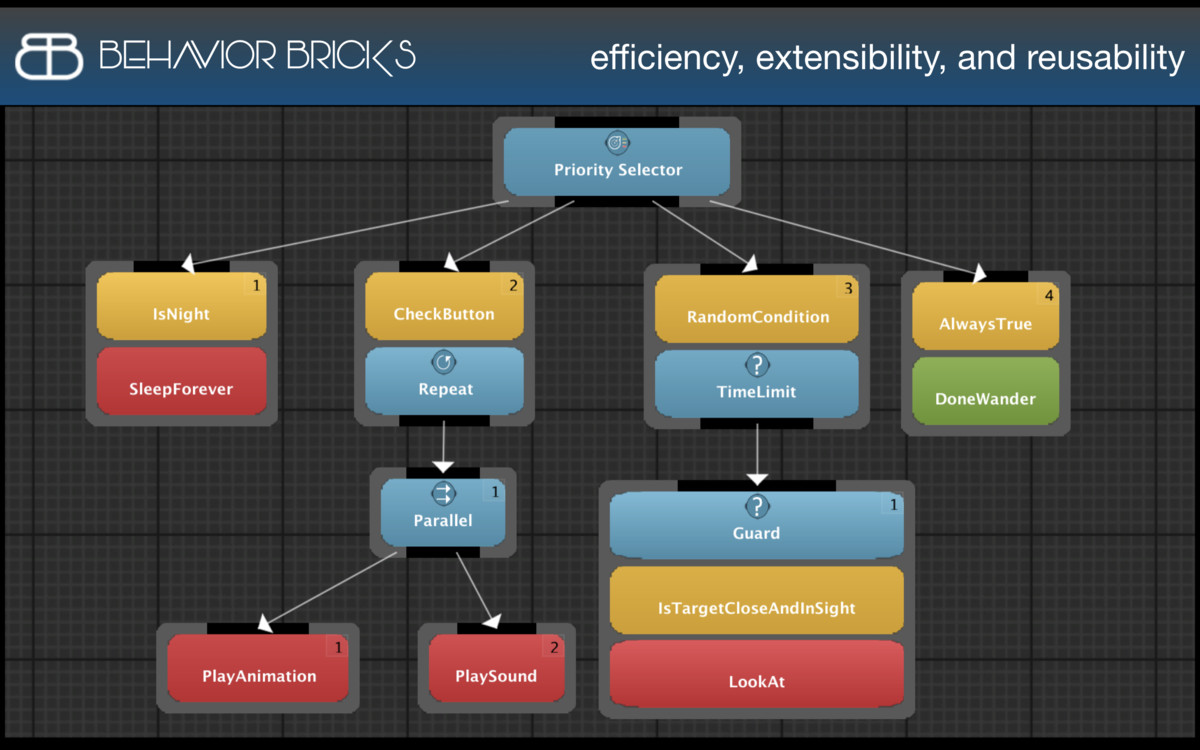
\includegraphics[width = 0.7\textwidth]{Imagenes/Behavior_Bricks.jpg}
	\caption{Ejemplo de uso de Behavior Bricks}
	\label{fig:BH_Figure}
\end{figure}
Un aspecto a destacar de esta herramienta es que es totalmente gratuita y fue desarrollada por \textit{PadaOne Games}\footnote{\url{https://www.padaonegames.com/}}, empresa asociada a la Universidad Complutense de Madrid.\\
\textit{Behavior Bricks} es una herramienta de scripting visual, por lo que favorece esa colaboración entre diseñadores y programadores que a veces es difícil de conseguir.\\
Otra particularidad de \textit{Behavior Bricks} es su modularidad, permite modificar cada una de las partes con muy poco acoplamiento entre ellas, lo que incita a su reutilización en distintos proyectos. Esta modularidad también permite que podamos tener un estado/comportamiento que sea en sí mismo un grupo de estados/comportamientos.\\
Esta herramienta hace hincapié en no ralentizar significativamente el rendimiento del juego, gracias a su optimización y la gestión de memoria la cual a veces es compartida entre estados/comportamientos para ahorrar recursos.\\

\subsection{Play Maker}
PlayMaker es un editor visual de FSM diseñado especialmente para artistas y diseñadores, ya que permite desarrollar IA sin necesidad de escribir código.

Su interfaz es altamente visual e intuitiva. Al crear una FSM, se genera automáticamente un estado inicial llamado \textit{START},como podemos ver en la Figura \ref{fig:PlayMaker_Figure}, seguido de un estado predeterminado llamado \textit{State 1}, al cual se transiciona al ejecutar \textit{Unity}. A partir de ahí, el usuario puede agregar más estados y definir eventos que permiten cambiar entre ellos según ciertas condiciones.

Una de sus principales ventajas es la facilidad con la que se pueden modificar los valores de los componentes de \textit{Unity}. Basta con arrastrar un componente a la pestaña \textit{State} para ajustar sus propiedades dentro de un estado determinado. Además, Play Maker proporciona una amplia colección de acciones predefinidas, como la detección de entrada de teclas, temporizadores y movimientos entre otros. Estas acciones pueden activar eventos que actúan como transiciones entre estados, facilitando la creación de mecánicas de juego complejas sin necesidad de programación.

Gracias a su flexibilidad y facilidad de uso, Play Maker es ideal para diseñar IAs, lógica de juego, animaciones, interacción con interfaces de usuario y prototipos rápidos, convirtiéndolo en una herramienta poderosa tanto para principiantes como para desarrolladores experimentados que buscan agilizar su flujo de trabajo. Otro punto fuerte de Play Maker es que permite que la herramienta sea escalable con scripts propios.

Play Maker está disponible en la \textit{asset store} de \textit{Unity}, aunque su precio hacer que desarrolladores con pocos recursos tengan que descartar esta opción, no deja de ser una herramienta usada ámpliamente por la comunidad de desarrolladores, habiendo sido utilizada en juegos como el aclamado por la crítica \textit{Hollow Night}\footnote{\url{https://hollowknight.fandom.com/wiki/Hollow_Knight_Wiki}}, \textit{Firewatch}\footnote{\url{https://www.firewatchgame.com/}} la aventura narrativa del estudio norteamericano Campo Santo o el juego de plataforma de los creadores de \textit{Limbo}, \textit{INSIDE}\footnote{\url{https://inside.fandom.com/wiki/Inside_Wiki}}.\\

\begin{figure}[h]
	\centering
	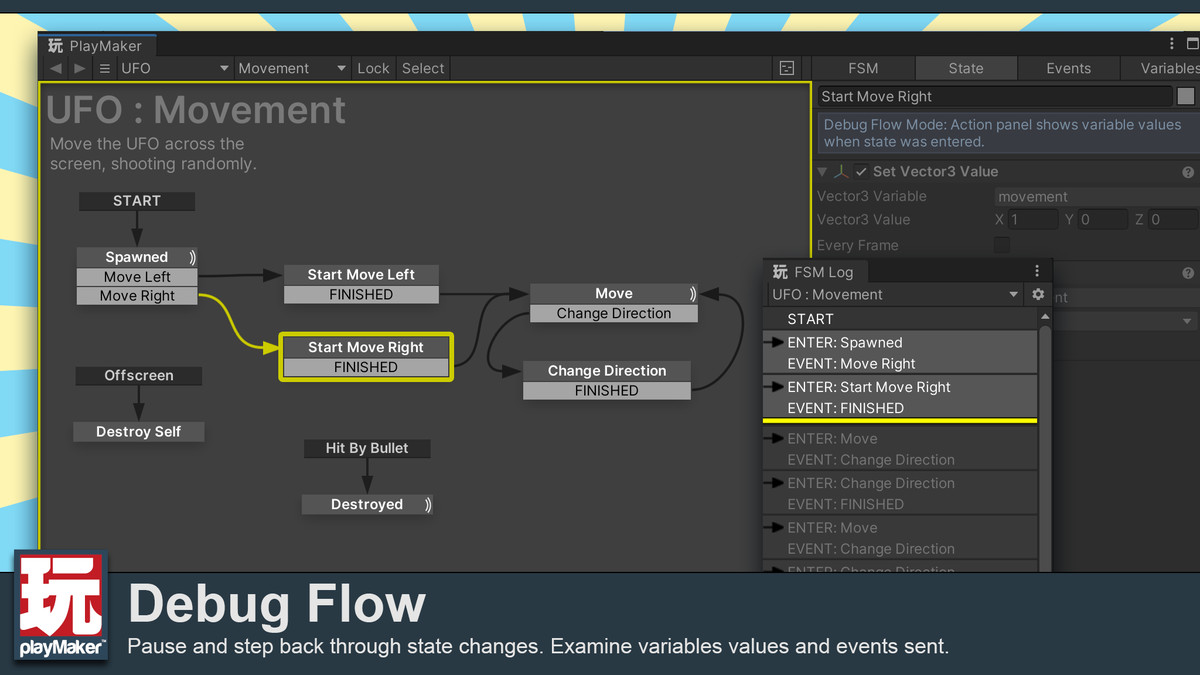
\includegraphics[width = 0.7\textwidth]{Imagenes/PlayMaker.jpg}
	\caption{Ejemplo de uso de Play Maker}
	\label{fig:PlayMaker_Figure}
\end{figure}

%\subsection{Animator}
\section{Motores de videojuegos}

Se ha abordado una serie de herramientas externas que se integran en el motor de videojuegos \textit{Unity}. Ahora se procederá a hablar sobre una serie de motores de videojuegos que ofrecen sustitutos para estas herramientas que vienen integrados en el propio motor lo que ayuda a que usuarios sin conocimientos de programación puedan usar con mayor facilidad estos motores.

%\subsection{Unity}
\subsection{Unreal Engine}
\textit{Unreal Engine}\footnote{\url{https://www.unrealengine.com/es-ES}}, desarrollado por \textit{Epic Games}\footnote{\url{https://www.epicgames.com/site/es-ES/home}}, es uno de los motores de videojuegos más potentes y utilizados en la industria de los videojuegos en títulos como la saga \textit{Hellblade}\footnote{\url{https://thehellblade.fandom.com/wiki/Hellblade:_Senua\%27s_Sacrifice}} o el éxito mundial \textit{Fornite}\footnote{\url{https://www.fortnite.com/?lang=es-ES}} y la versión más actual es Unreal Engine 5 que cuenta, entre otras cosas, con \textit{Lumen}, un sistema de iluminación global dinámica o la mejora sustancial del sistema de simulación de físicas \textit{Chaos}.\\
A pesar de que permite la programación en C++, también ofrece un sistema visual llamado Blueprints, diseñado para que cualquier persona, sin conocimientos de programación, pueda crear videojuegos completos mediante una interfaz gráfica intuitiva.

El sistema de Blueprints funciona de manera similar a un lenguaje de programación visual basado en nodos. En lugar de escribir código manualmente, el usuario conecta bloques de lógica (Figura \ref{fig:BluePrints_Figure}) para definir comportamientos, interacciones y mecánicas dentro del juego. Esto permite crear desde movimientos de personajes y mecánicas de combate hasta sistemas complejos de inteligencia artificial y físicas sin necesidad de escribir una sola línea de código.\\
Cabe destacar que se pueden crear Blueprints en caso de que sea necesario.
\begin{figure}[h]
	\centering
	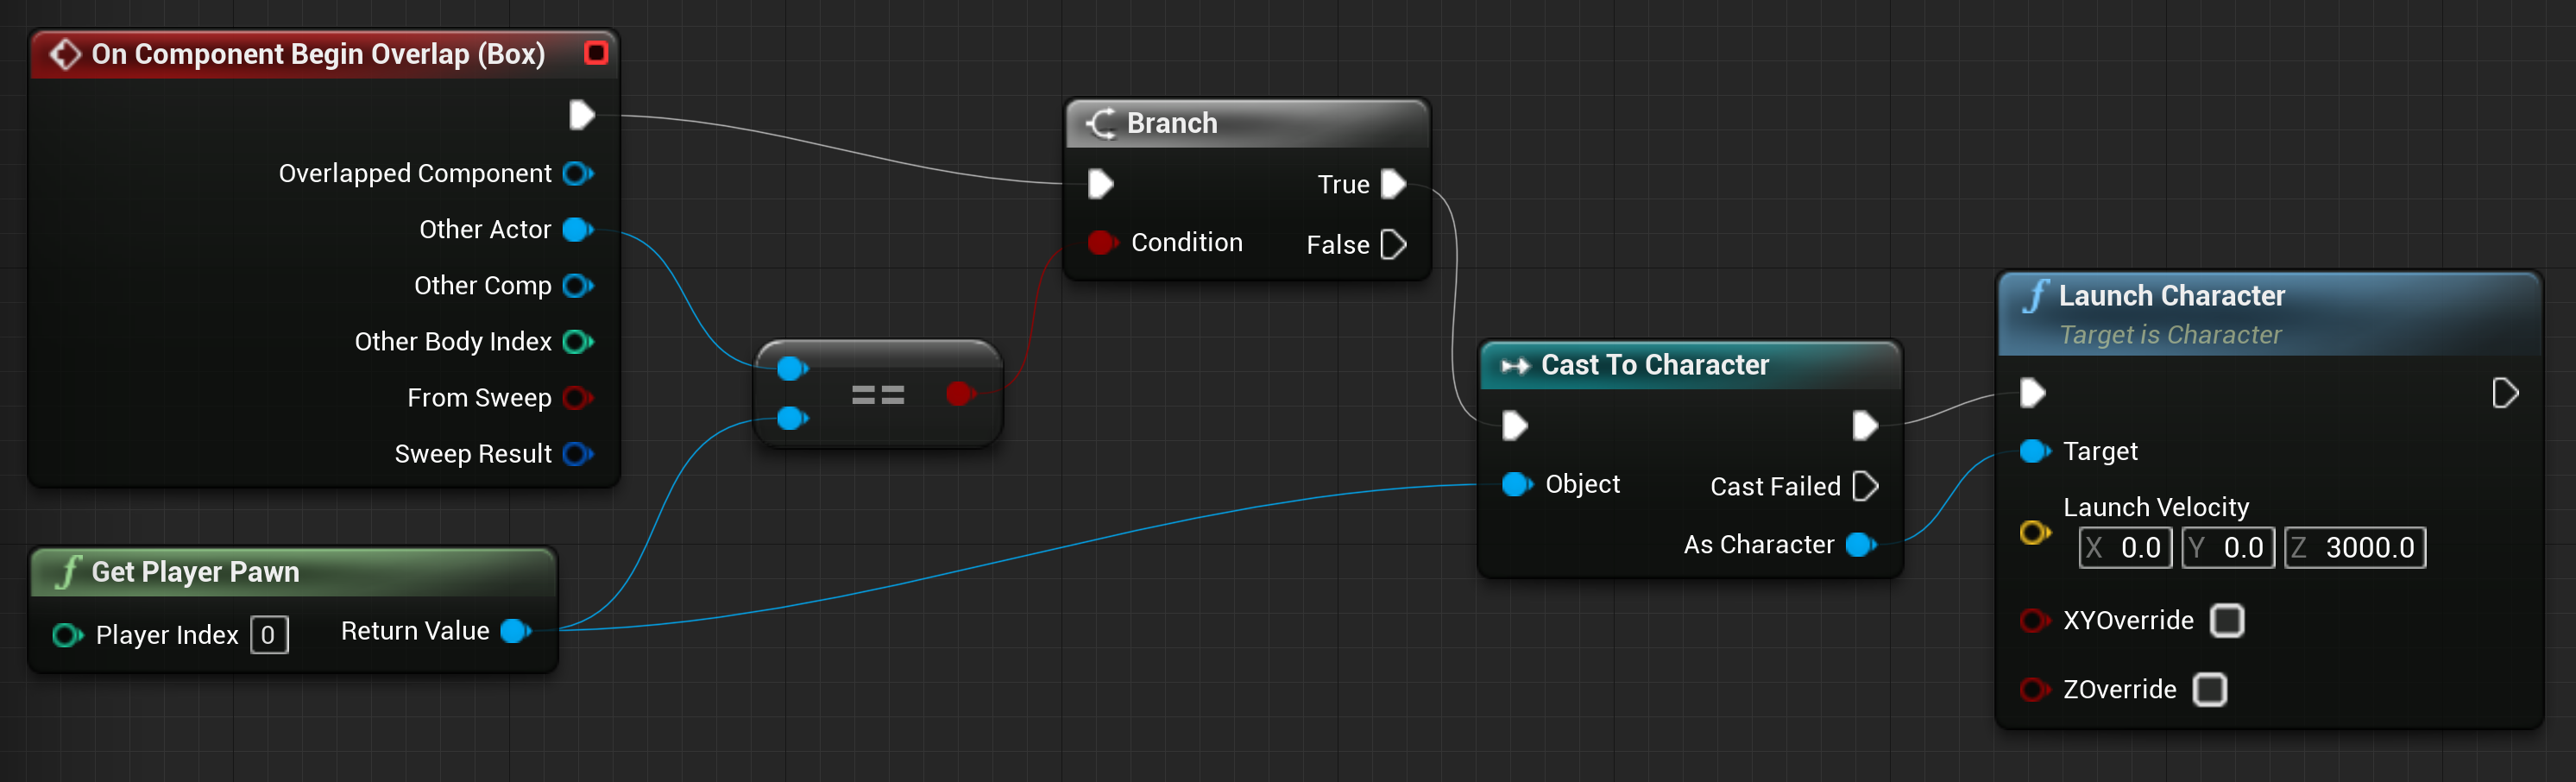
\includegraphics[width = 0.7\textwidth]{Imagenes/Blueprints.png}
	\caption{Blueprints en Unreal Engine}
	\label{fig:BluePrints_Figure}
\end{figure}

Además, Unreal Engine incluye un conjunto de herramientas preconfiguradas que facilitan el desarrollo, como sistemas de animación, iluminación, renderizado de alta calidad y físicas avanzadas. Gracias a estas características, cualquier usuario puede desarrollar videojuegos en 2D y 3D de manera accesible y rápida, sin necesidad de aprender un lenguaje de programación tradicional.

Si se compara con otros motores como Unity, Unreal Engine destaca por su calidad gráfica y su sistema visual más robusto. Mientras que en Unity se requiere programación para acceder a ciertas funciones avanzadas, en Unreal es posible construir mecánicas complejas únicamente con Blueprints. Esto lo convierte en una opción ideal para desarrolladores novatos que buscan facilidad de uso sin sacrificar potencia y flexibilidad.

Un punto negativo de Unreal Engine con respecto a Unity es la necesidad de recursos hardware que tiene para poder usarlo sin ningún tipo de ralentizaciones ni crasheos fortuitos, necesitando equipos muy potentes para que el desarrollo sea ameno o utilizar versiones anteriores de Unreal Engine.

Gracias a los Blueprints, cualquier persona puede diseñar enemigos, implementar IA, construir niveles interactivos y desarrollar mecánicas de juego avanzadas sin tocar código. 
\subsection{Godot}

Godot, desarrollado por Juan Linietsky y Arenanet, es un motor de videojuegos de código abierto que ha ganado popularidad por su accesibilidad, flexibilidad y sencillez. Ofrece una plataforma poderosa para desarrollar videojuegos tanto en 2D como en 3D, y uno de sus mayores atractivos es que está diseñado para ser fácil de usar sin necesidad de tener conocimientos avanzados de programación.

A diferencia de otros motores como Unreal Engine o Unity, Godot permite el desarrollo de videojuegos con una interfaz intuitiva, pero también brinda herramientas más accesibles para aquellos que no desean escribir código. Su sistema de GDScript, un lenguaje propio diseñado específicamente para ser fácil de aprender y usar, facilita la creación de juegos sin necesidad de un conocimiento profundo de programación. GDScript es similar a Python (comparten sintaxis y tipado dinámico), lo que lo hace accesible y amigable para desarrolladores noveles.

Además, Godot ofrece un sistema de nodos (Figura \ref{fig:Godot_Figure}) que permite a los usuarios crear y organizar elementos dentro de su juego de una manera visual y modular. Cada nodo en Godot representa una pieza o componente del juego (como personajes, objetos, cámaras, luces, etc.), y los desarrolladores pueden organizarlos jerárquicamente. Esta estructura es extremadamente flexible, ya que cualquier nodo puede ser programado o configurado para comportarse de acuerdo con el flujo del juego, lo que simplifica la creación de interacciones y lógicas complejas.
\begin{figure}[h]
	\centering
	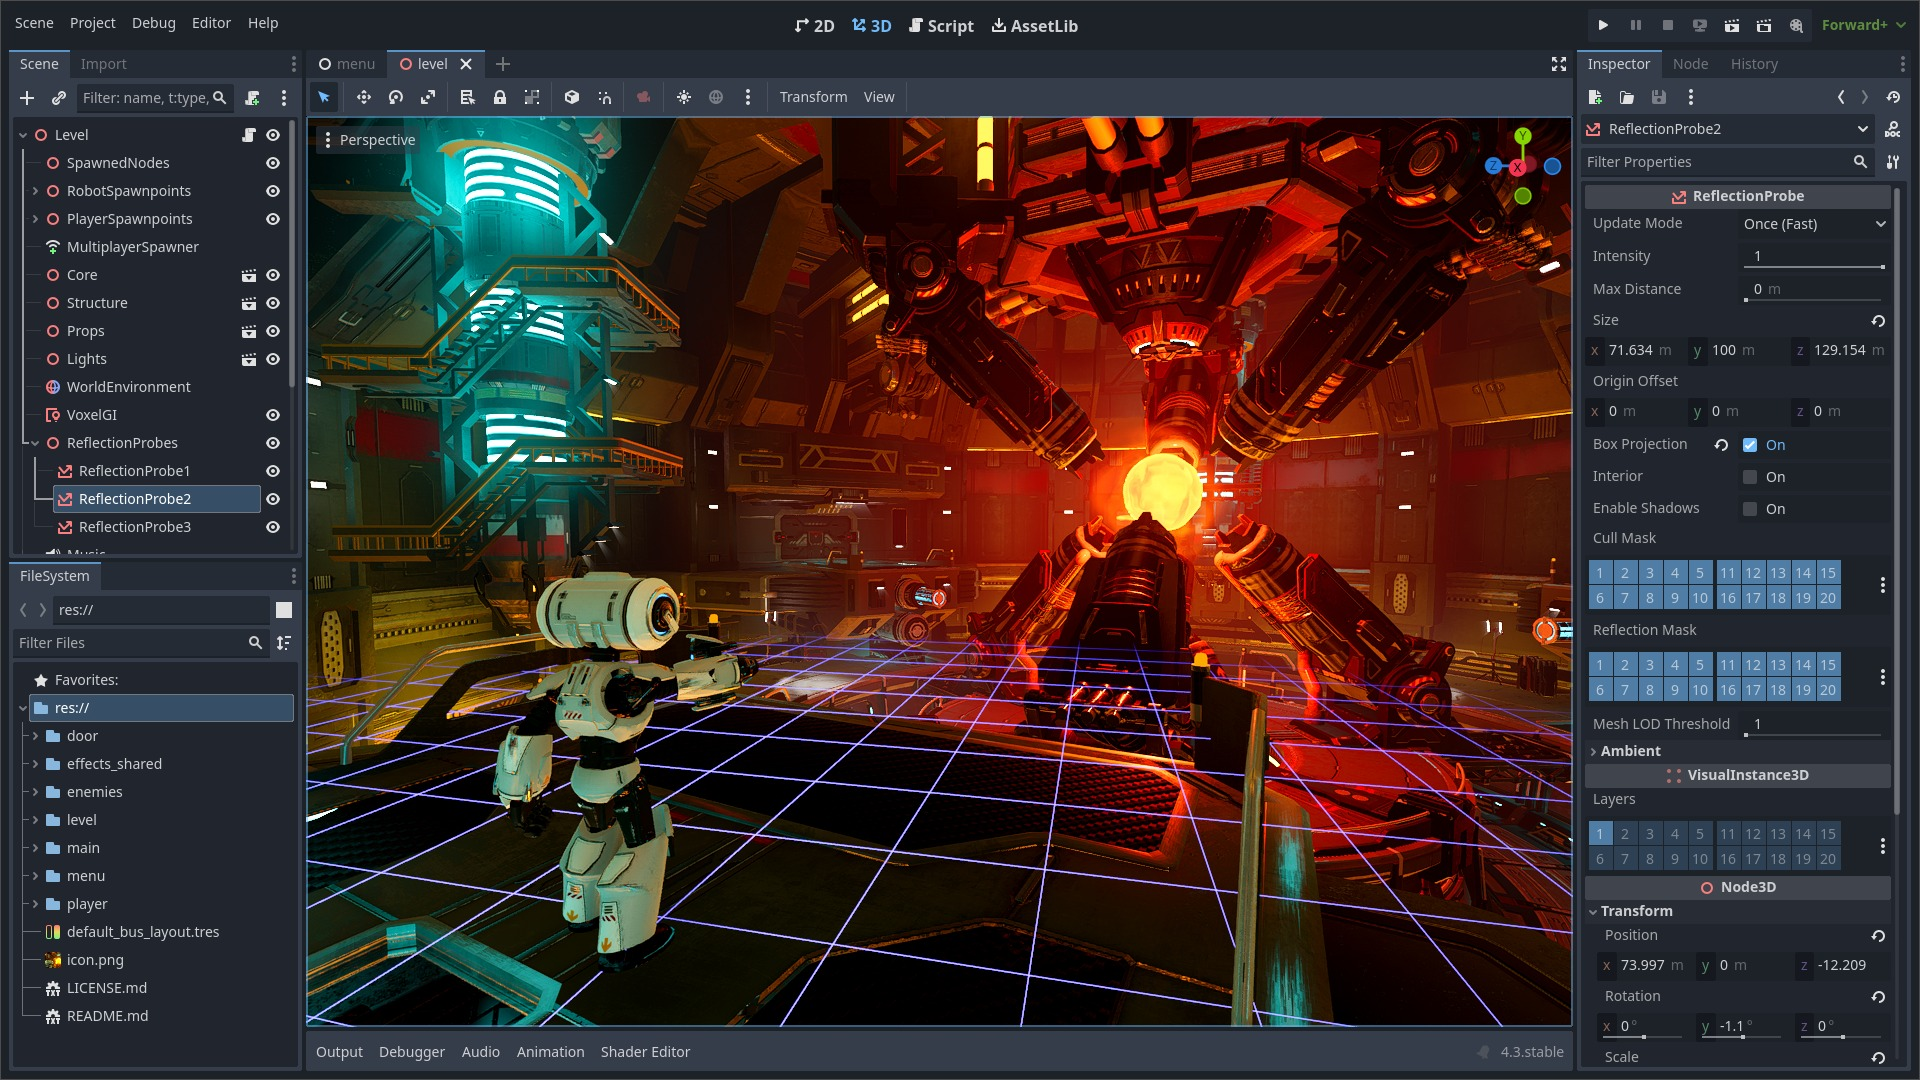
\includegraphics[width = 0.7\textwidth]{Imagenes/Godot.jpg}
	\caption{Interfaz de Godot}
	\label{fig:Godot_Figure}
\end{figure}

Para aquellos que prefieren una experiencia más visual y menos enfocada en la programación, Godot también incluye un sistema de "VisualScript" (Figura \ref{fig:Godot_VisualScript_Figure}), un lenguaje visual basado en nodos que permite desarrollar mecánicas sin escribir código. Similar a los sistemas de programación visual en otros motores como Unreal Engine. Este sistema ha sido eliminado del núcleo de Godot a partir de la versión 4.0 del motor aunque en lanzamientos futuros VisualScript será re-implementado como una extensión\footnote{\url{https://docs.godotengine.org/es/3.5/tutorials/scripting/visual_script/index.html}}.

\begin{figure}[h]
	\centering
	\includegraphics[width = 0.7\textwidth]{Imagenes/VisualScriptGodot.pdf}
	\caption{Sistema VisualScript en Godot}
	\label{fig:Godot_VisualScript_Figure}
\end{figure}
Godot también destaca por ser un motor muy optimizado para el desarrollo de juegos en 2D, proporcionando una serie de herramientas específicas para este tipo de desarrollo, como un sistema de mallas 2D, animaciones, efectos y un conjunto de físicas dedicadas al mundo 2D. De esta manera, los desarrolladores pueden crear juegos con un rendimiento óptimo, incluso para dispositivos de baja gama, y con un flujo de trabajo ágil.

Comparado con otros motores como Unreal Engine o Unity, Godot se distingue por su flexibilidad y ligereza. No requiere licencias ni regalías, lo que lo convierte en una excelente opción para proyectos indie como el roguelite \textit{Brotato}\footnote{\url{https://brotato.wiki.spellsandguns.com/Brotato_Wiki}} y desarrolladores independientes. También es especialmente potente para aquellos interesados en el desarrollo de juegos 2D, ya que ofrece herramientas específicamente diseñadas para este propósito, algo en lo que otros motores como Unity o Unreal Engine no se enfocan tanto.

Gracias a su accesibilidad y herramientas poderosas, Godot permite a desarrolladores sin experiencia en programación crear juegos completos, desde mecánicas simples hasta sistemas complejos, sin necesidad de escribir código avanzado. Esta facilidad de uso, combinada con un motor robusto y libre, hace que Godot sea una opción popular para quienes buscan comenzar en el mundo del desarrollo de videojuegos o aquellos que desean una solución completamente gratuita y personalizable para sus proyectos.
\subsection{GameMaker}
\subsection{Construct 3}
\section{Conclusiones}
-----------------------------------------------------\\
En el estado de la cuestión es donde aparecen gran parte de las referencias bibliográficas del trabajo. Una de las formas más cómodas de gestionar la bibliografía en {\LaTeX} es utilizando \textbf{bibtex}. Las entradas bibliográficas deben estar en un fichero con extensión \textit{.bib} (con esta plantilla se proporciona el fichero biblio.bib, donde están las entradas referenciadas más abajo). Cada entrada bibliográfica tiene una clave que permite referenciarla desde cualquier parte del texto con los siguiente comandos:

\begin{itemize}
\item Referencia bibliografica con cite: \cite{ldesc2e}
\item Referencia bibliográfica con citep: \citep{notsoshort}
\item Referencia bibliográfica con citet: \citet{latexAPrimer}
\end{itemize}

Es posible citar más de una fuente, como por ejemplo \citep{latexCompanion,LaTeXLamport,texKnuth}

Después, \LaTeX se ocupa de rellenar la sección de bibliografía con las entradas \textbf{que hayan sido citadas} (es decir, no con todas las entradas que hay en el .bib, sino sólo con aquellas que se hayan citado en alguna parte del texto).

Bibtex es un programa separado de latex, pdflatex o cualquier otra cosa que se use para compilar los .tex, de manera que para que se rellene correctamente la sección de bibliografía es necesario compilar primero el trabajo (a veces es necesario compilarlo dos veces), compilar después con bibtex, y volver a compilar otra vez el trabajo (de nuevo, puede ser necesario compilarlo dos veces). 
